%%%%%%%%%%%%%%%%%%%%%%%%%%%%%%%%%%%%%%%%%
% Make sure to set your name, legi number and url to the right git branch.
\newcommand{\hmwkAuthorName}{IDIL KANPOLAT} % Your name
\newcommand{\hmwkAuthorLegi}{16-931-107} % Your name
\newcommand{\hmwkGitBranch}{YOUR GIT BRANCH} % Your name
%
%%%%%%%%%%%%%%%%%%%%%%%%%%%%%%%%%%%%%%%%%
%----------------------------------------------------------------------------------------
%	PACKAGES AND OTHER DOCUMENT CONFIGURATIONS
%	Skip this
%----------------------------------------------------------------------------------------
\documentclass{article}
\usepackage{amsmath}
\usepackage{graphicx} % Required to insert images
\usepackage{float}
\usepackage{caption}


\usepackage{amsfonts}
\usepackage{fancyhdr} % Required for custom headers
\usepackage{lastpage} % Required to determine the last page for the footer
\usepackage{extramarks} % Required for headers and footers

\usepackage{lipsum} % Used for inserting dummy 'Lorem ipsum' text into the template
% Margins
\topmargin=-0.45in
\evensidemargin=0in
\oddsidemargin=0in
\textwidth=6.5in
\textheight=9.0in
\headsep=0.25in 
\linespread{1.1} % Line spacing
% Set up the header and footer
\pagestyle{fancy}
\lhead{\hmwkAuthorName} % Top left header
\chead{\hmwkClass\ \hmwkTitle} % Top center header
\rhead{\firstxmark} % Top right header
\lfoot{\lastxmark} % Bottom left footer
\cfoot{} % Bottom center footer
\rfoot{Page\ \thepage\ of\ \pageref{LastPage}} % Bottom right footer
\renewcommand\headrulewidth{0.4pt} % Size of the header rule
\renewcommand\footrulewidth{0.4pt} % Size of the footer rule
\setlength\parindent{0pt} % Removes all indentation from paragraphs
%----------------------------------------------------------------------------------------
%	DOCUMENT STRUCTURE COMMANDS
%	Skip this
%----------------------------------------------------------------------------------------
% Header and footer for when a page split occurs within a problem environment
\newcommand{\enterProblemHeader}[1]{
\nobreak\extramarks{#1}{#1 continued on next page\ldots}\nobreak
\nobreak\extramarks{#1 (continued)}{#1 continued on next page\ldots}\nobreak
}
% Header and footer for when a page split occurs between problem environments
\newcommand{\exitProblemHeader}[1]{
\nobreak\extramarks{#1 (continued)}{#1 continued on next page\ldots}\nobreak
\nobreak\extramarks{#1}{}\nobreak
}
\setcounter{secnumdepth}{0} % Removes default section numbers
\newcounter{homeworkProblemCounter} % Creates a counter to keep track of the number of problems
\newcommand{\homeworkProblemName}{}
\newenvironment{homeworkProblem}[1][Problem \arabic{homeworkProblemCounter}]{ % Makes a new environment called homeworkProblem which takes 1 argument (custom name) but the default is "Problem #"
\stepcounter{homeworkProblemCounter} % Increase counter for number of problems
\renewcommand{\homeworkProblemName}{#1} % Assign \homeworkProblemName the name of the problem
\section{\homeworkProblemName} % Make a section in the document with the custom problem count
\enterProblemHeader{\homeworkProblemName} % Header and footer within the environment
}{
\exitProblemHeader{\homeworkProblemName} % Header and footer after the environment
}
\newcommand{\problemAnswer}[1]{ % Defines the problem answer command with the content as the only argument
\noindent\framebox[\columnwidth][c]{\begin{minipage}{0.98\columnwidth}#1\end{minipage}} % Makes the box around the problem answer and puts the content inside
}
\newcommand{\homeworkSectionName}{}
\newenvironment{homeworkSection}[1]{ % New environment for sections within homework problems, takes 1 argument - the name of the section
\renewcommand{\homeworkSectionName}{#1} % Assign \homeworkSectionName to the name of the section from the environment argument
\subsection{\homeworkSectionName} % Make a subsection with the custom name of the subsection
\enterProblemHeader{\homeworkProblemName\ [\homeworkSectionName]} % Header and footer within the environment
}{
\enterProblemHeader{\homeworkProblemName} % Header and footer after the environment
}
   
%----------------------------------------------------------------------------------------
%	NAME AND CLASS SECTION
%	Skip this
%----------------------------------------------------------------------------------------
\newcommand{\hmwkTitle}{Locally Linear Embedding} % Assignment title
\newcommand{\hmwkDueDate}{Monday,\ March\ 6th,\ 2017} % Due date
\newcommand{\hmwkClass}{SLT coding exercise\ \#1} % Course/class
\newcommand{\hmwkClassTime}{Mo 16:15} % Class/lecture time
\newcommand{\hmwkClassInstructor}{} % Teacher/lecturer
%----------------------------------------------------------------------------------------
%	TITLE PAGE
%	Skip this
%----------------------------------------------------------------------------------------
\title{
\vspace{2in}
\textmd{\small{\hmwkClass}}\\
\textmd{\textbf{\hmwkTitle}}\\
\small{https://gitlab.vis.ethz.ch/vwegmayr/slt-coding-exercises}\\
\normalsize\vspace{0.1in}\small{Due\ on\ \hmwkDueDate}
%\vspace{0.1in}\large{\textit{\hmwkClassInstructor\ \hmwkClassTime}}
\vspace{3in}
}
\author{
\hmwkAuthorName\\
\hmwkAuthorLegi
}
\date{ } % Insert date here if you want it to appear below your name
\begin{document}
\maketitle
%----------------------------------------------------------------------------------------
%	TABLE OF CONTENTS
%	Skip this
%----------------------------------------------------------------------------------------
%\setcounter{tocdepth}{1} % Uncomment this line if you don't want subsections listed in the ToC
\newpage
\tableofcontents
\newpage
%----------------------------------------------------------------------------------------
%	SECTIONS
%	Now you are in the right hood
%----------------------------------------------------------------------------------------
\begin{homeworkProblem}[The Model]
The model section is intended to allow you to recapitulate the essential ingredients used in \hmwkTitle. Write down the \textit{necessary} equations to specify \hmwkTitle\ and and shortly explain the variables that are involved. This section should only introduce the equations, their solution should be outlined in the implementation section.\newline
\vspace{10pt}
\problemAnswer{ % Answer

With LLE we are calculating the low dimensional embedding of our dataset considering the neighbours of the data points. The aim is to find the weights of the mapping by minimizing the error function defined and after fixing the weights finding the low dimensional vectors by minimizing the related error function.\\
\begin{center}
$V:=\{X_1, X_2, ... X_N\}$  is a finite subset of $ R^D$ and $N(X_i):=\{X \in V|X \text{ is a neighbour of } X_i\}$.\\~\\
 
 Find $W_{ij}$ that minimizes\\ $E(W) = \sum_{i}(X_i-\sum_{j} W_{ij}X_j)^2$ subject to 
$\sum_{j} W_{ij} = 1$ and $for X_j \notin N(X_i),  W_{ij}=0$\\ ~\\

For fixed $W$ find $U:=\{Y_1, Y_2, ... Y_N\} \in  R^d, d \ll D$ that minimizes\\
 $E(Y) = \sum_{i}(Y_i-\sum_{j} W_{ij}Y_j)^2$  subject to $\sum_{i} Y_i = 0$ and $\sum_{i}Y_i^T Y_i = \mathbb{I} $ 

\end{center}
}
\end{homeworkProblem}
\clearpage
%----------------------------------------------------------------------------------------
\begin{homeworkProblem}[The Questions]
This is the core section of your report, which contains the tasks for this exercise and your respective solutions. Make sure you present your results in an illustrative way by making use of graphics, plots, tables, etc. so that a reader can understand the results with a single glance. Check that your graphics have enough resolution or are vector graphics. Consider the use of GIFs when appropriate.\newline
Hard limit: Two pages
\begin{homeworkSection}{(a) Get the data}
For this exercise we will work with the MNIST data set. In order to learn more about it and download it, go to http://yann.lecun.com/exdb/mnist/.
\end{homeworkSection}
\begin{homeworkSection}{(b) Locally linear embedding}
Implement the LLE algorithm and apply it to the MNIST data set. Provide descriptive visualizations for 2D \& 3D embedding spaces. Is it possible to see clusters?
\end{homeworkSection}
\begin{homeworkSection}{(c) Cluster structure}
Investigate the cluster structure of the data. Can you observe block structures in the $M$ matrix (use matrix plots)? Also plot the singular values of $M$. Do you notice something?
Can you think of ways to determine the optimal embedding dimension?
\end{homeworkSection}
\begin{homeworkSection}{(d) Nearest Neighbors}
Investigate the influence of the choice of how many nearest neighbors you take into account. Additionally, try different metrics to find the nearest neighbors (we are dealing with images!).
\end{homeworkSection}
\begin{homeworkSection}{(e) Linear manifold interpolation}
Assume you pick some point in the embedding space. How can you map it back to the original (high dimensional) space? Investigate how well this works for points within and outside the manifold (does it depend on the dimensionality of the embedding space?) Try things like linearly interpolating between two embedding vectors and plot the sequence of images along that line. What happens if you do that in the original space?
\end{homeworkSection}
\vspace{10pt}
\problemAnswer{ % Answer
\title{\large\textbf{(b) Locally linear embedding}}\\
I have applied LLE to 3000 points of MNIST test set due to time constraint. The results for k=5 and k=30  nearest neighbours and for 2 dim and 3 dim cases can be seen below. In the graphs bellow the numbers represent the class labels. In both cases it is not really possible to observe a distinguishable cluster structure but overlapping clusters. There are labels with distinguishable behaviour such as class 0 for    'k=5, 2D, 3000 points' case. 
}
\begin{figure}[H]
\begin{minipage}[b]{.5\textwidth}
\centering
\hspace*{-3cm}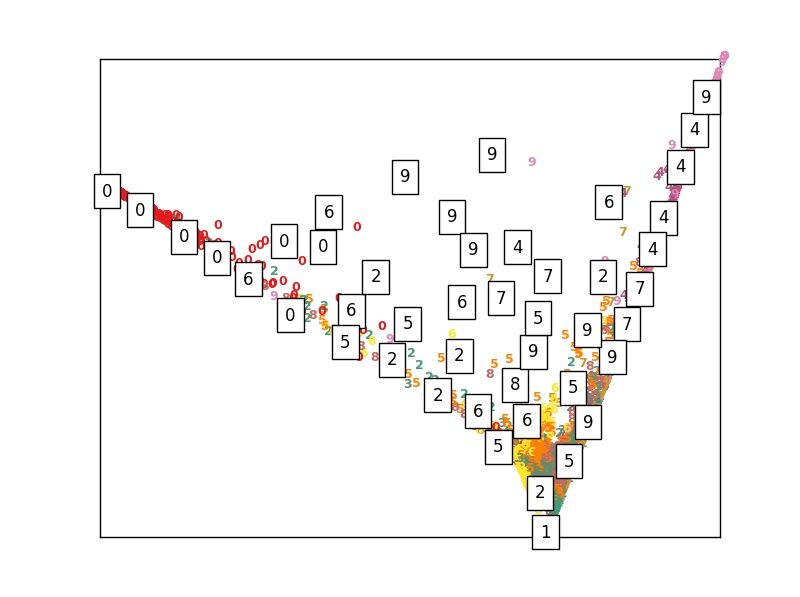
\includegraphics[width=1.2\textwidth]{5_2D_3000.jpeg}
\hspace*{-3cm}\caption{Embedded vectors for k=5, 2D, 3000 points}
\end{minipage}
\hfill
\begin{minipage}[b]{.4\textwidth}
\centering
\hspace*{-1cm}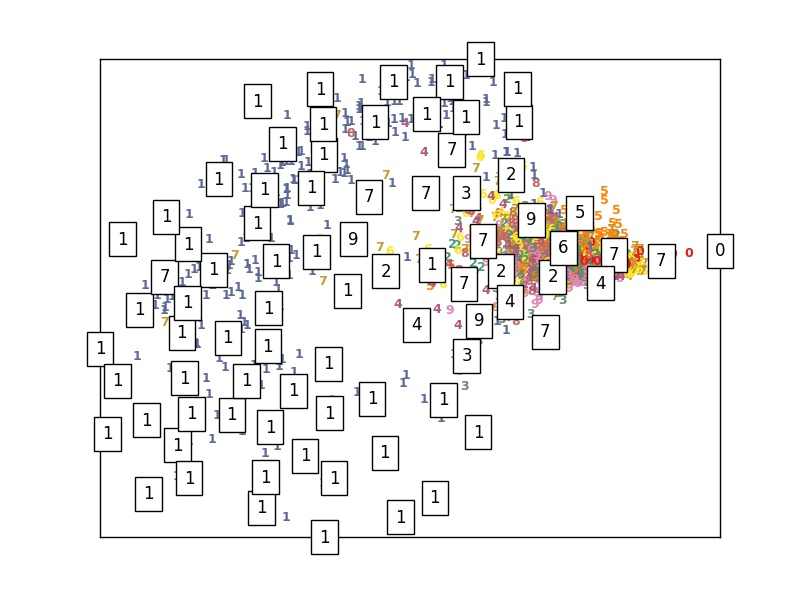
\includegraphics[width=1.5\textwidth]{30_2D_3000.jpeg}
\caption{Embedded vectors for k=30, 2D, 3000 points}
\end{minipage}
\end{figure}

\begin{figure}[H]
\begin{minipage}[b]{.5\textwidth}
\centering
\hspace*{-3cm}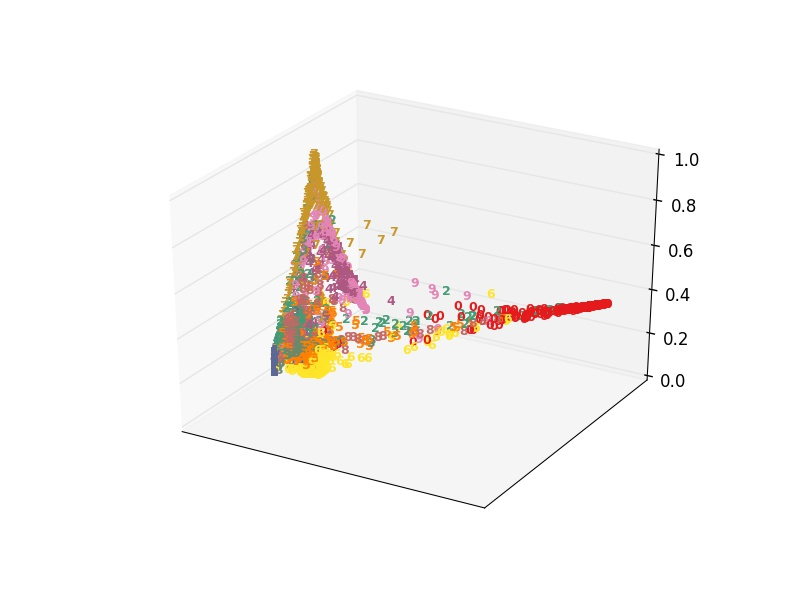
\includegraphics[width=1.5\textwidth]{5_3D_3000.jpeg}
\caption{Embedded vectors for k=5, 3D, 3000 points}
\end{minipage}
\hfill
\begin{minipage}[b]{.4\textwidth}
\centering
\hspace*{-3cm}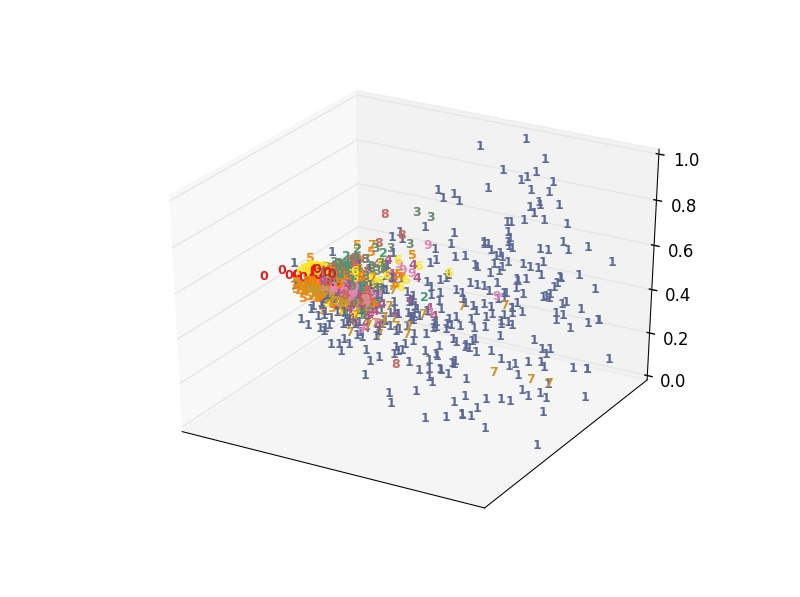
\includegraphics[width=2\textwidth]{30_3D_3000.jpeg}
\caption{Embedded vectors for k=30, 3D, 3000 points}
\end{minipage}
\end{figure}

\problemAnswer{ % Answer
\title{\large\textbf{(c) Cluster structure}}\\
In the exercise we have seen that minimizing the error corresponds to finding the d eigenvectors of $M =  (\mathbb{I}-W)^T(\mathbb{I}-W)$ with the smallest eigenvalues that are not equal to zero. We can decide on the number d with respect to the eigenvalues that are small enough. The figure below represents the $M$ matrix, where the diagonal elements contain the information and the rest of the elements are mostly sparse. The second figure is a plot of the eigenvalues which might help deciding on the dimension of the mapped space.  
}

\begin{figure}[H]
\begin{minipage}[b]{.5\textwidth}
\centering
\hspace*{-3cm}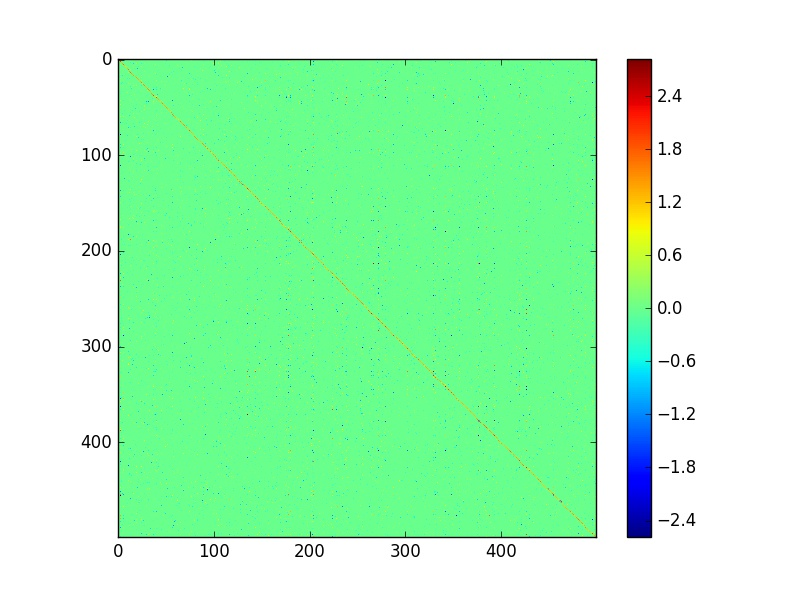
\includegraphics[width=1.5\textwidth]{M.jpeg}
\caption{M matrix for k=30, 800 points}
\end{minipage}
\hfill
\begin{minipage}[b]{.4\textwidth}
\centering
\hspace*{-2cm}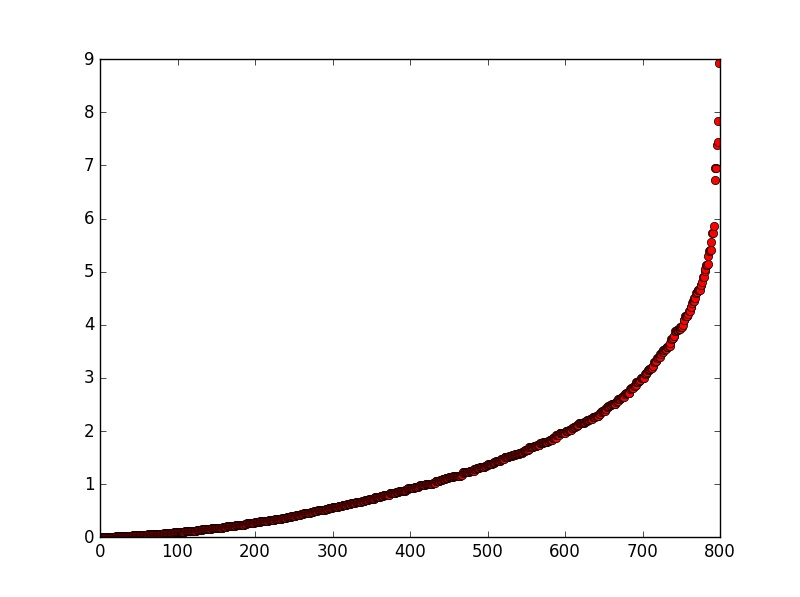
\includegraphics[width=1.5\textwidth]{eigenValues.jpeg}
\caption{Eigenvalues of M matrix for k=30, 800 points}
\end{minipage}
\end{figure}

\problemAnswer{ % Answer
\title{\large\textbf{(d) Nearest Neighbors}}\\
The mapping is repeated for different number of nearest neighbours. From the figures we can see that a small number such as k=2 will not be efficient to reflect the global structure of the dataset, whereas increasing k can cause us to lose its nonlinear character\cite{1}. 
}

\begin{figure}[H]

\centering
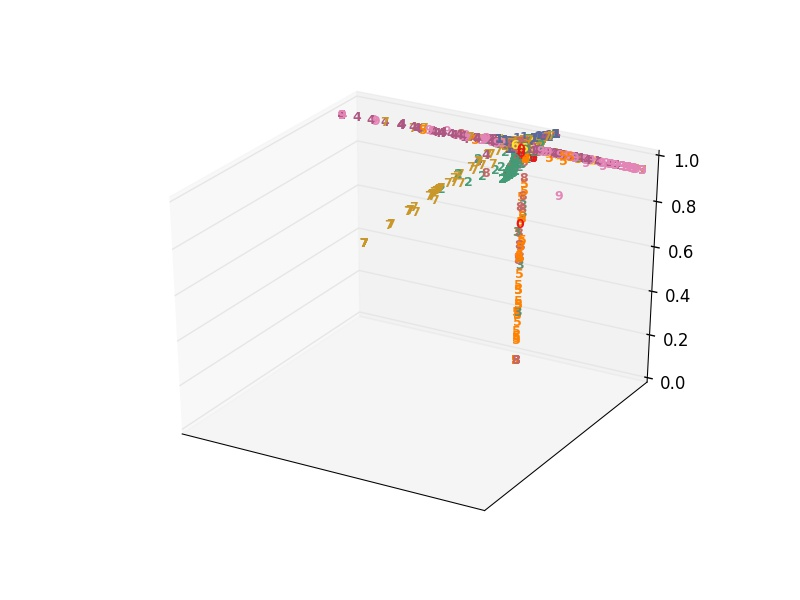
\includegraphics[width=.4\textwidth]{2_3D_3000.jpg}\hfill
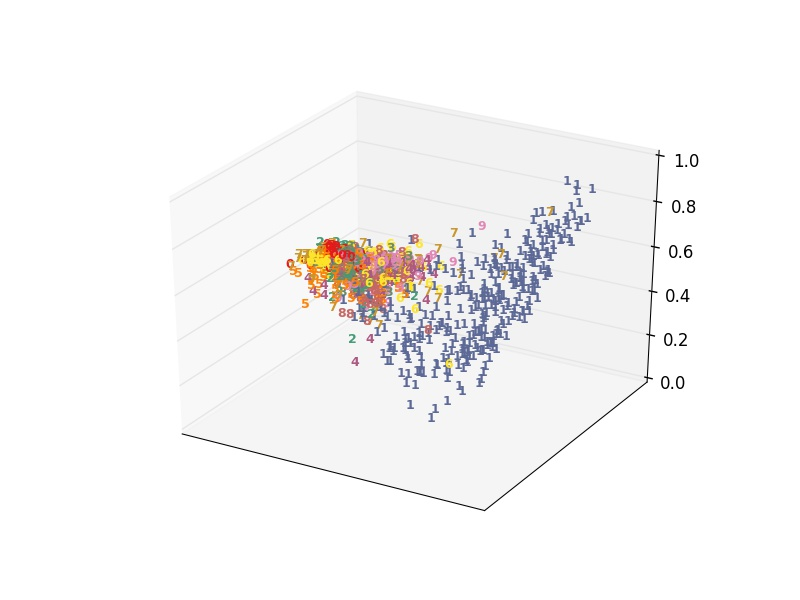
\includegraphics[width=.4\textwidth]{50_3D_3000.jpg}\hfill
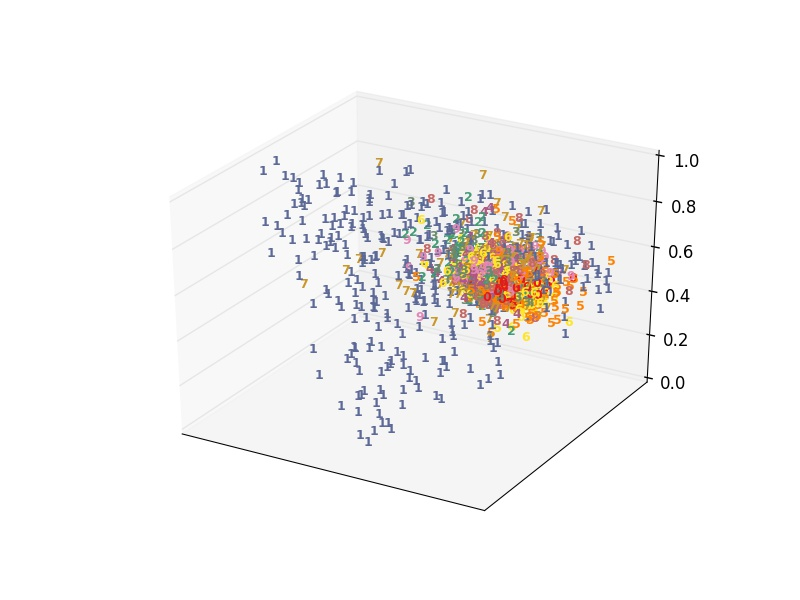
\includegraphics[width=.4\textwidth]{100_3D_3000.jpg}

\caption{Embedded vectors for k= 2, 50, 100, 3D, 3000 points}
\label{fig:figure3}

\end{figure}

\problemAnswer{ % Answer
\title{\large\textbf{(e) Linear manifold interpolation}}\\

}

\end{homeworkProblem}
\clearpage
%----------------------------------------------------------------------------------------
\begin{homeworkProblem}[The Implementation]
In the implementation section you give a concise insight to the practical aspects of this coding exercise. It mainly mentions the optimization methods used to solve the model equations. Did you encounter numerical or efficiency problems? If yes, how did you solve them?
Provide the link to your git branch of this coding exercise.\newline
Hard limit: One page\\
\vspace{10pt}
\problemAnswer{ % Answer
I have used  scikit-learn for implementation mostly. The code is slow for cases with high number of data points or high number of nearest neighbours.  To eliminate these problems I have worked with 3000 points in most of the cases. I believe the main bottleneck is the nearest neighbour calculation. \\
16-931-107\slash1\_locally\_linear\_embedding} 
\end{homeworkProblem}
\clearpage
%----------------------------------------------------------------------------------------
\begin{homeworkProblem}[Your Page]
Your page gives you space to include ideas, observations and results which do not fall into the categories provided by us. You can also use it as an appendix to include things which did not have space in the other sections.\newline
No page limit.\\
\vspace{10pt}
\problemAnswer{ % Answer 
16-931-107\slash1\_locally\_linear\_embedding

}
\end{homeworkProblem}
 \begin{thebibliography}{1}
  \bibitem{1}Juliana Valencia-Aguirre, Andrés Álvarez-Mesa {\em Automatic Choice of the Number of Nearest Neighbors in Locally Linear Embedding} CIARP, pp 77-84, 2009.
\end{thebibliography}
\clearpage
\end{document}